%!TEX root = emnlp2016.tex

Foreign embassies of the United States government communicate with one
another and with the U.S. State Department through diplomatic cables.
The National Archive collects these cables in a corpus, which traces
the (declassified) diplomatic history of the United States. The corpus
contains, for example, over two million cables sent between 1973 and
1978.

Most of these cables describe diplomatic ``business as usual,'' such
as arrangements for visiting officials, recovery of lost or stolen
passports, or obtaining lists of names for meetings and
conferences. For example, the embassies sent 8,635 cables during the
week of April 21, 1975. Here is one, selected at random:
\begin{shaded*} \tt{Hoffman, UNESCO Secretariat, requested info from
PermDel concerning an official invitation from the USG
RE subject meeting scheduled 10--13 JUNE 1975, Madison,
Wisconsin.  Would appreciate info RE status of action to
be taken in order to inform Secretariat.  Hoffman communicating
with Dr.~John P.~Klus RE list of persons to be invited.}
\end{shaded*}

But, hidden in the corpus are also cables about important diplomatic
events---the cables and events that are most interesting to
historians, political scientists, and journalists. For example, during
that same week, the U.S. was in the last moments of the Vietnam war
and, on April 30, 1975, lost its hold on Saigon. This marked the
end of the war and a mass exodus of refugees. Here is one of the cables
about this event:
\begin{shaded*}
  \tt{GOA program to move Vietnamese Refugees to Australia
  is making little progress and probably will not cover more than
  100-200 persons.  Press comment on smallness of program has
  recognized difficulty of getting Vietnamese out of Saigon, but
  ``Canberra Times'' Apr 25 sharply critical of government's
  performance.  [...]
  %Opposition continues to attack smallness of program,
  %but seems concerned, as does government, with scoring
  %point of domestic political importance.  With Parliament in
  %recess for next three weeks and Prime Minister on trip, issue
  %may attract less attention.
  Labor government clearly hopes whole
  matter will somehow disappear.}
\end{shaded*}

% cheating by putting this here...
\begin{figure*}[ht]
\centering
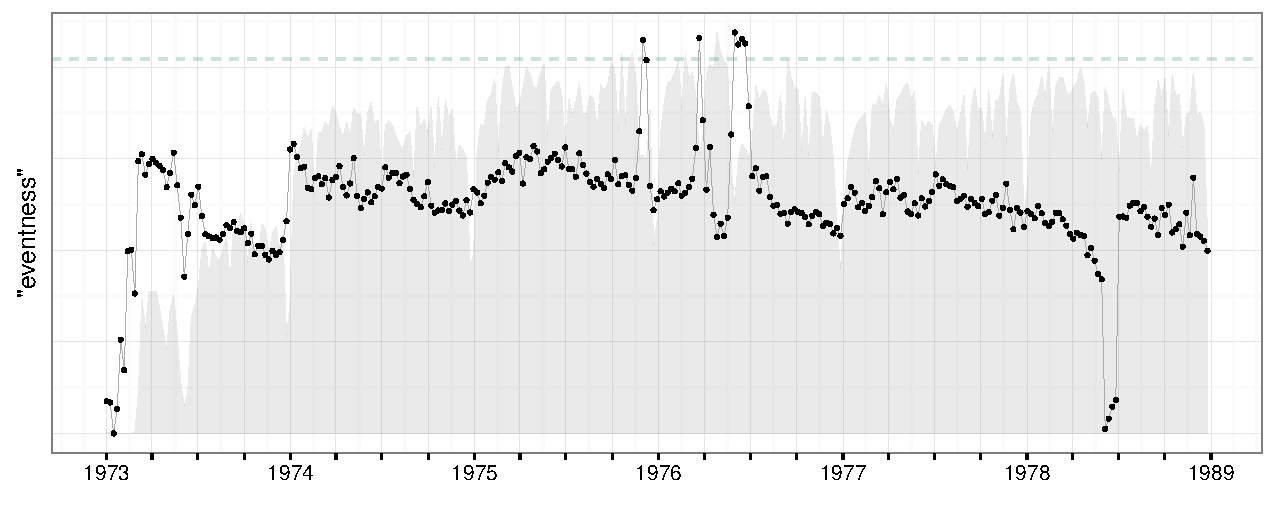
\includegraphics[width=\linewidth]{fig/cables_events.pdf}
\caption{Measure of ``eventness,'' or time interval impact on cable content (Eq.~\ref{eq:eventness}).  Grey background indicates the number of cables sent over time.  This comes from the model fit we discuss in \Cref{sec:eval}.  Capsule successful detects real-world events from National Archive diplomatic cables.}
\label{fig:cables_events}
\end{figure*}

Our goal in this paper is to develop a tool to help historians,
political scientists, and journalists wade through corpora of
documents to find potentially significant events and the primary
sources around them. We present \textit{Capsule}, a probabilistic
model for detecting and characterizing important events, such as the
fall of Saigon, in large corpora of historical communication, such as
diplomatic cables from the 1970s.

\Cref{fig:cables_events} illustrates Capsule's analysis of two million
cables from the National Archives' corpus. The \mbox{$y$-axis}
represents ``eventness,'' a loose measure of how strongly a week's
cables deviate from typical diplomatic ``business as usual'' to
discuss some matter that is common to many embassies. (We describe
this measure of ``eventness'' in detail in \cref{sec:model}.)

% THIS PARAGRAPH IS UNTOUCHED...
The figure shows that Capsule detects many of the important moments
during this five-year span, including the Air France hijacking and
Israeli rescue operation ``Operation Entebbe'' (June 27--July 4,
1976), and the fall of Saigon (April 30, 1975). It also identifies
other moments, such as the U.S. sharing lunar rocks with other
countries (March 21, 1973) and the death of Mao Tse-tung (Sept. 9,
1976). Broadly speaking, Capsule gives a picture of the diplomatic
history of these five years; it identifies and characterizes moments
and source material that might be of interest to a historian.

The intuition behind Capsule is this: Embassies write cables
throughout the year, usually describing typical diplomatic business,
such as visits from government officials. Sometimes, however,
important events occur, such as the fall of Saigon, that pull
embassies away from their typical activities and lead them to write
cables that discuss these events and their consequences. Capsule
therefore operationalizes an ``event'' as a moment in history when
multiple embassies deviate from their usual topics of discussion and
each embassy deviates in the same way.

Capsule embeds this intuition into a Bayesian model that uses latent
variables to encode what ``business as usual'' means for each embassy,
to characterize the events of each week, and to identify the cables
that discuss those events. Given a corpus of cables, the corresponding
posterior distribution of the latent variables provides a filter for
the cables that isolates important moments in diplomatic
history. \Cref{fig:cables_events} depicts the mean of this posterior
distribution.

We present the Capsule model in \cref{sec:model}, providing both a
formal model specification and guidance on how to use the model to
detect and characterize real-world events. In \cref{sec:valid}, we
validate Capsule using simulated data, and in \cref{sec:eval},
we use it to analyze over two million U.S. State Department
cables. Although we describe Capsule in the context of diplomatic
cables, it is suitable for exploring any corpus with the same
underlying structure: text (or other discrete multivariate data)
generated over time by known entities. This includes email, consumer
behavior, social media posts, and opinion articles.

\section{Related Work}

% I prefer having this as a stand-alone section

%\parhead{Related work.}

We first review previous work on automatic event detection and other
related concepts, to contextualize our approach in general and Capsule
in particular.

% While Capsule uses text documents and associated metadata as input, event detection is often performed with univariate input data.  In this context, bursts that deviate from typical behavior (e.g., noisy constant or a repeating pattern) can define an event \cite{kleinberg2003bursty,ihler2007learning}; Poisson Processes~\cite{Kingman:1993} are often used to model events under this definition.  Alternatively, events can be construed as ``change points'' to mark when typical observations shift semi-permanently from one value to another~\cite{guralnik1999event}.

In both univariate and multivariate settings, analysts often want to
predict whether or not rare events will
occur~\cite{weiss1998learning,das2008anomaly}. In contrast, Capsule is
intended to help analysts explore and understand their data; our goal
is human interpretability rather than prediction or forecasting.

Events can be construed as either anomalies---temporary deviations
from usual behavior---or ``changepoints'' that mark persistent shifts
in usual behavior~\cite{guralnik1999event,adams2007bayesian}. We focus
on events as anomalies.

% Text is often used in event detection, as it is an abundant source of data.
% In some applications, documents themselves are considered to be observed events~\cite{mccallum1998comparison,peng2007event}, or events are predetermined and tracked through the documents~\cite{yang2000improving,VanDam:2012}.  We are interested in detecting \emph{unobserved} events which can be characterized by patterns in the data.
%\newpage % note:when using hyperref, references can be split between
%pages!

Event detection in the context of news
articles~\cite{zhao2012novel,zhao2007temporal,zhang2002novelty,li2005probabilistic,wang2007mining,allan1998line}
and social media
posts~\cite{VanDam:2012,lau2012line,jackoway2011identification,sakaki2010earthquake,reuter2012event,becker2010learning,sayyadi2009event}
usually means identifying clusters of documents. For news, the goal is
to create new clusters as novel stories appear, without distinguishing
between typical content and rare events; for social media, the goal is
to identify rare events, but the resultant methods are intended for
short documents, and are not appropriate for longer documents that
contain information about a variety of subjects.

Many existing methods for detecting events from text focus on
individual vocabulary terms, often weighted by tf-idf
values~\cite{fung2005parameter,kumaran2004text,brants2003system,das2011dynamic,zhao2007temporal,zhao2012novel}.
We characterize events by bursts in groups of terms.
% Because language is high dimensional, using terms as features limits
% scalability.

Although groups of terms can be summarized
directly~\cite{peng2007event,chakrabarti2011event,gao2012joint}, topic
models~\cite{Blei:2012} provide a way to automatically identify groups
of related terms and reduce the dimensionality of text
data. Researchers have previously used topic models to detect events
mentioned in social media posts~\cite{lau2012line,dou2012leadline} and
to find posts relevant to particular, monitored
events~\cite{VanDam:2012}. Capsule uses topics to characterize both
typical diplomatic content and potentially significant events.

In addition to modeling text over time, researchers have also used
spatial
information~\cite{Neill:2005,mathioudakis2010identifying,liu2011using}
and information about authors~\cite{zhao2007temporal} and news
outlets~\cite{wang2007mining} to enhance event detection. We rely on
author information to characterize diplomatic ``business as usual''
for each embassy.

Event detection is closely related to detecting and characterizing
relationships between
entities~\cite{schein2015bayesian,linderman2014discovering,das2011dynamic}. Capsule
can trivially use sender--receiver pairs instead of authors, and the
model specification can be tailored to reflect network structure.

Finally, there are connections between Capsule and recent work on
Poisson processes. In particular, we can interpret Capsule as a
collection of related discrete-time Poisson processes with random
intensity measures. Further, marginalizing out the event strengths
% IS THIS RIGHT?
(described in \cref{sec:model_spec}) reveals that the use of a
vocabulary term by one embassy can ``excite'' the use of that term by
another. This suggests a close relationship to Hawkes
processes~\cite{hawkes1971spectra}.


% TODO: cite he2015hawkestopic
